\section{Closure of Event Selection}
\label{sec:GBJ2:AODD3PD}

To check the event selection, two separate implementations of the analysis were performed by the Manchester and UCL groups.
One of these analyses was carried out using the ATLAS AOD data format, whilst the other used the ATLAS D3PD format.
Figure \ref{GBJ2:AODD3PD:gap_njet} shows (a) the  gap fraction and (b) the  average number of jets in the rapidity region as a function of \dy{}.
Figure \ref{GBJ2:AODD3PD:dphi} shows the \dphi{} distribution for inclusive events for a dijet separation, \dy{}, of (a) 2-3 and (b) 4-5. 
All four plots show very good agreement between the AOD and D3PD implementations of the analysis.
The small disagreements arise from the data compression algorithms that store the data information.
This effects mainly the jet energies and the effect is much smaller than the JES uncertainty.


\begin{figure}
\centering
        \begin{subfigure}[b]{0.5\textwidth}
                \centering
                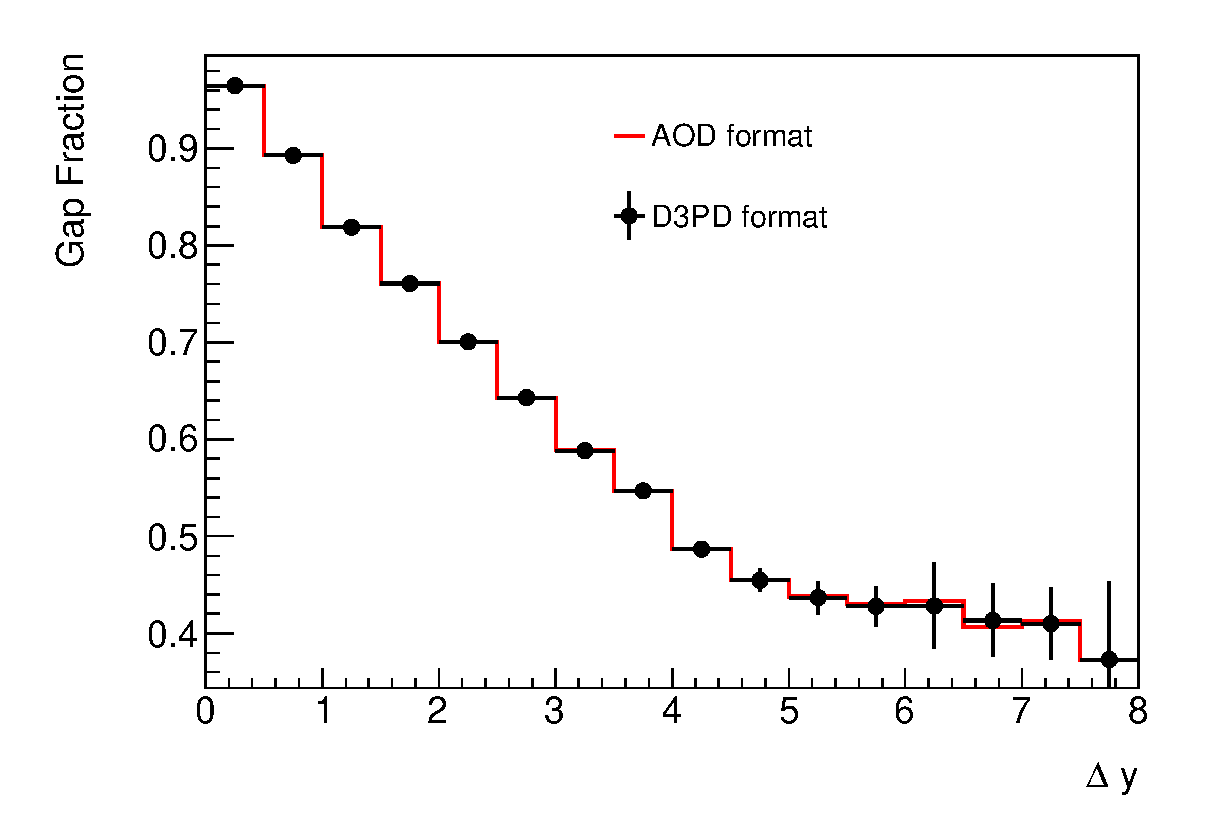
\includegraphics[height = 6cm,width=\textwidth]{figures/GBJ2/AODD3PD/Comp_GapFraction_deltaY.eps}
        \end{subfigure}%
        \begin{subfigure}[b]{0.5\textwidth}
                \centering
                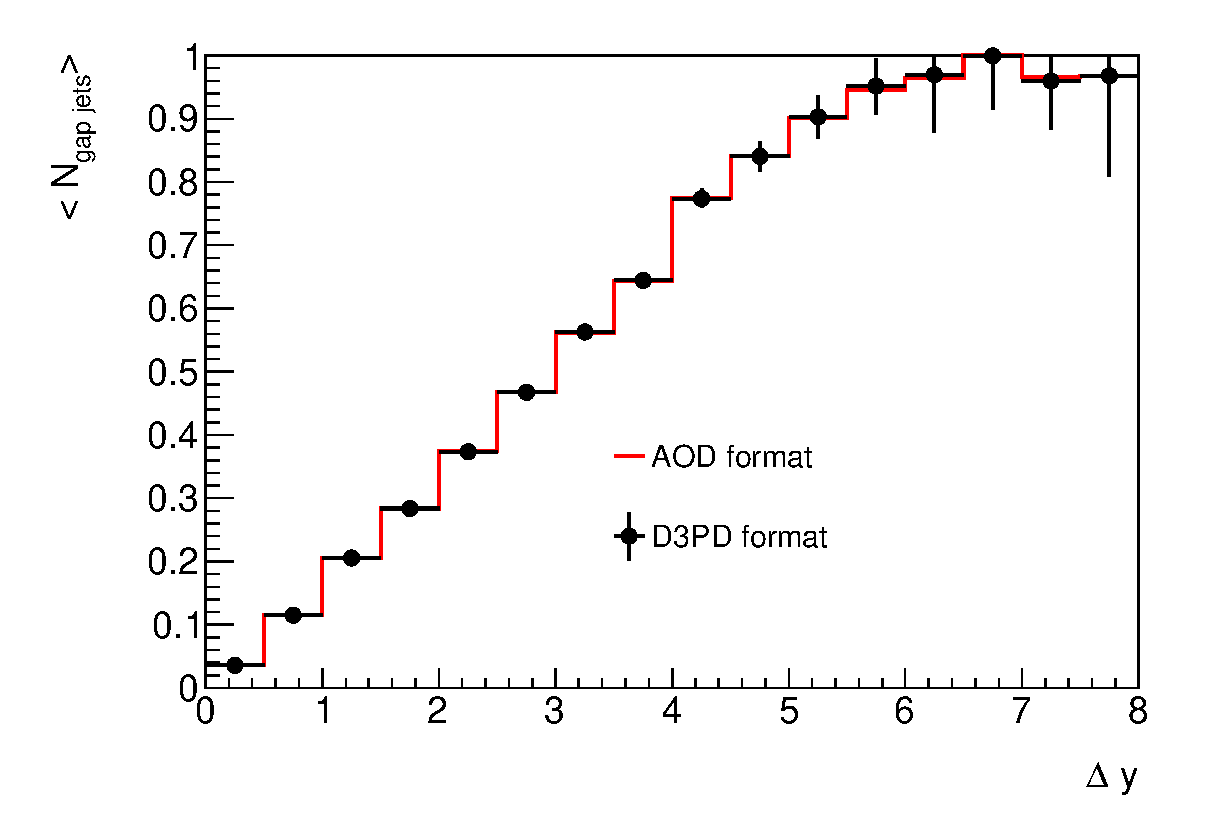
\includegraphics[height = 6cm,width=\textwidth]{figures/GBJ2/AODD3PD/Comp_prof_deltaY_njets.eps}
        \end{subfigure}%
\caption[Comparison of gap fraction and mean number of jets between AOD data format and D3PD data format]{
(a) Gap fraction and (b) average number of jets in the rapidity region as a function of dijet separation, \dy{}, for 2010 uncorrected data from the AOD (red) and D3PD (black) data formats.
\label{GBJ2:AODD3PD:gap_njet}}
\end{figure}


\begin{figure}
\centering
        \begin{subfigure}[b]{0.5\textwidth}
                \centering
                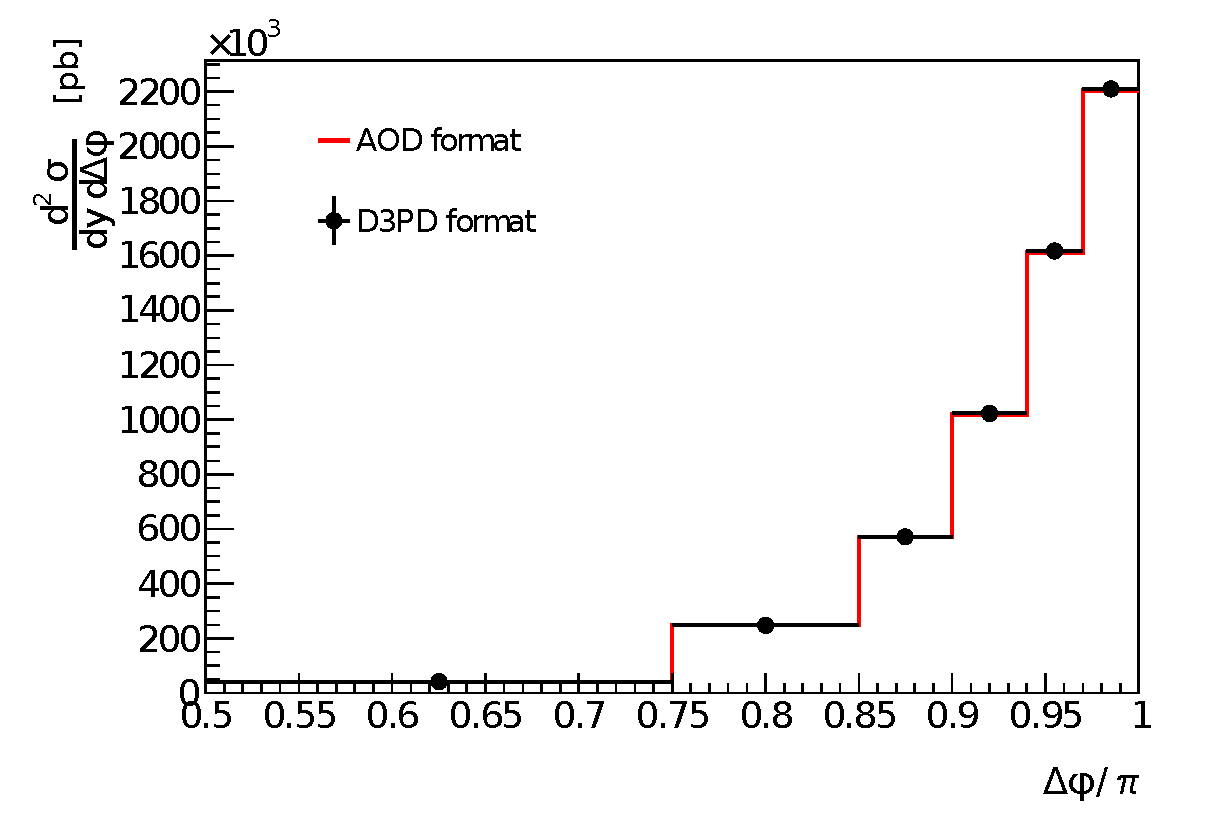
\includegraphics[height = 6cm,width=\textwidth]{figures/GBJ2/AODD3PD/Comp_dPhi__2_3-Edit.eps}
        \end{subfigure}%
        \begin{subfigure}[b]{0.5\textwidth}
                \centering
                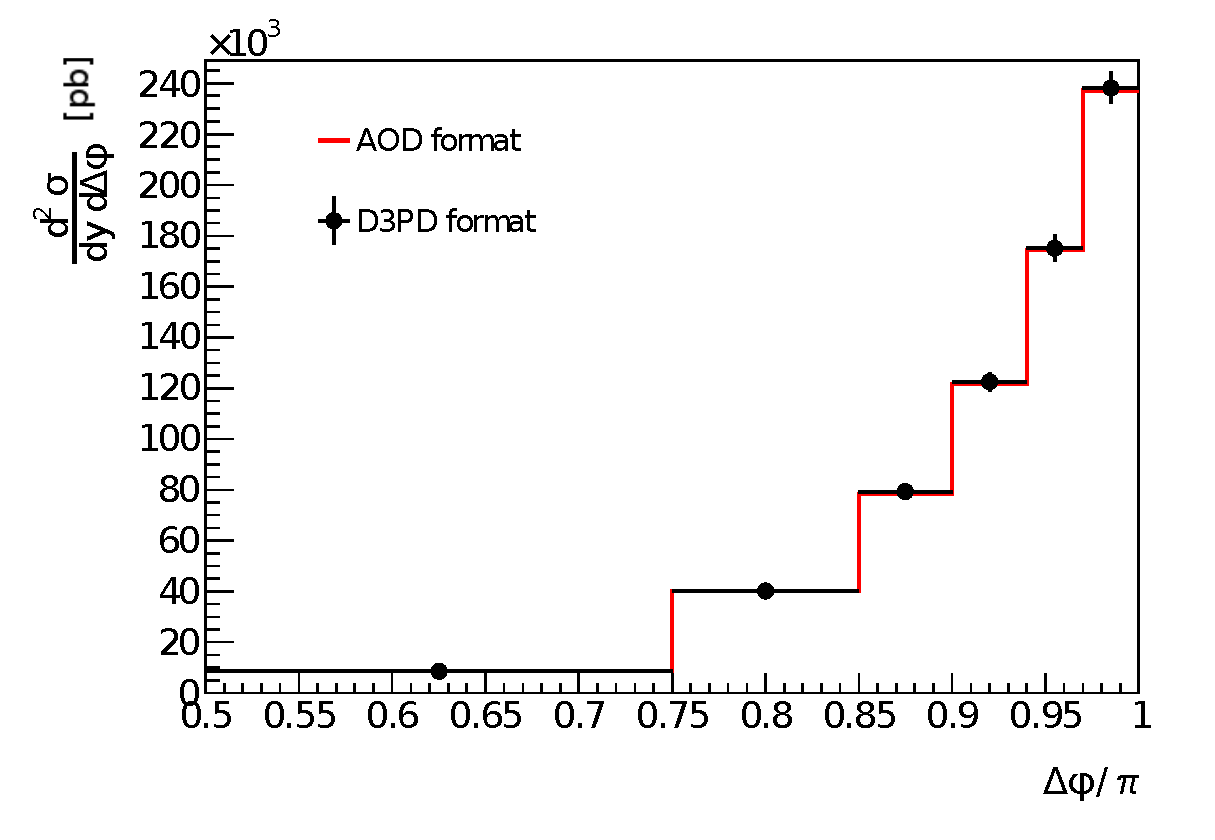
\includegraphics[height = 6cm,width=\textwidth]{figures/GBJ2/AODD3PD/Comp_dPhi__4_5-Edit.eps}
        \end{subfigure}%
\caption[Comparison of \dphiDist{} between AOD data format and D3PD data format]{
\dphiDist{} for inclusive events for a dijet separation of (a) $2<\dy{}<3$ and (b) $4<\dy{}<5$ for 2010 uncorrected data from the AOD (red) and D3PD (black) data formats.
\label{GBJ2:AODD3PD:dphi}}
\end{figure}

